\section{Introduction}
\label{sec:intro}
Spatial reasoning from visual observations is fundamental for intelligent systems interacting with physical environments. Vision-language models have achieved remarkable progress in understanding 3D spatial relationships from images, enabling applications in robotic manipulation~\cite{bohg2014robot}, augmented reality~\cite{azuma1997survey}, and autonomous navigation~\cite{boninfont2008visual}. Recent approaches extract metric spatial information using monocular depth estimation~\cite{yang2024depth} and scene understanding~\cite{ravi2024sam} to ground natural language queries about object positions, distances, and orientations.

Despite this progress, single-view spatial reasoning faces an intrinsic limitation: the projection from 3D to 2D is inherently lossy. Depth ordering becomes ambiguous when objects lack strong monocular cues, scale and distance trade off in producing identical image appearances, and occlusions hide spatial relationships. Methods such as SpatialVLM~\cite{chen2024spatialvlm}, SpatialRGPT~\cite{cheng2024spatialrgpt}, and SpatialReasoner~\cite{ma2025spatialreasoner} address this through increasingly sophisticated reasoning pipelines, yet remain fundamentally constrained by the information available in a single view.

We approach spatial reasoning from a multi-view perspective, leveraging the geometric constraint that consistent 3D structure must explain observations from multiple viewpoints. Novel views are synthesized using MVGenMaster~\cite{ren2025mvgenmaster}, a generative model that produces photorealistic images without the artifacts of geometric projection methods. The model is trained on paired views with view-aware chain-of-thought supervision, learning to integrate complementary geometric information for spatial inference.

A key finding of our work is that multi-view training confers benefits only when inference maintains the same paradigm. Models trained on synthesized multi-view data but evaluated on single images fail to outperform simpler baselines, revealing a distribution mismatch between training and testing conditions. When both training and inference utilize dual-view inputs, our approach achieves 60.1\% accuracy on 3DSRBench, demonstrating that multi-view consistency provides a viable path toward robust spatial understanding.

This work makes three contributions. First, we propose a multi-view spatial reasoning framework as an alternative to reinforcement learning approaches. While SpatialReasoner~\cite{ma2025spatialreasoner} achieves state-of-the-art performance through chain-of-thought supervision followed by GRPO-based refinement, our approach instead leverages geometric consistency across synthesized viewpoints, achieving comparable accuracy without reinforcement learning. Second, we introduce view-aware chain-of-thought supervision with coordinate transformation, ensuring that spatial descriptions remain consistent with each synthesized viewpoint. Third, we provide empirical analysis demonstrating the necessity of train-test alignment for realizing multi-view benefits---models trained on multi-view data but evaluated on single images fail to improve, an insight with implications for future multi-view learning approaches.

\begin{figure*}[ht!]
\centering
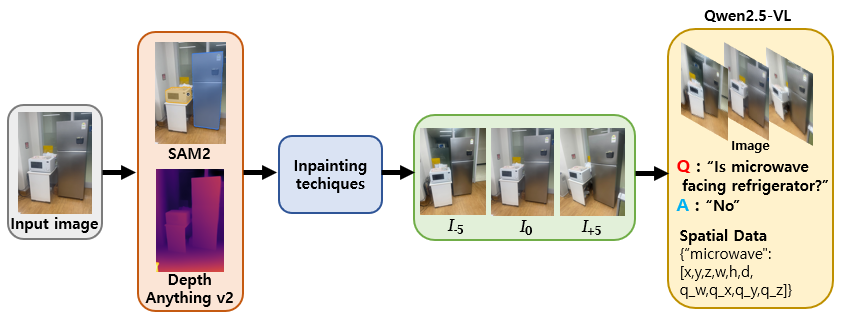
\includegraphics[width=0.8\textwidth]{figures/dummy.png}
\caption{Overview of multi-view spatial reasoning pipeline. Given an input image, MVGenMaster synthesizes a rotated view at $10^\circ$ azimuth. Both views are presented to the model with explicit viewpoint annotations. Chain-of-thought supervision incorporates coordinate transformation to ensure spatial descriptions remain consistent with each view's perspective. During inference, the same dual-view paradigm is maintained for train-test alignment.}
\label{fig:view-synthesis-overview}
\end{figure*}
